
\section{Avalanche involving a shock wave}

We consider an avalanche involving a shock wave.
This problem is similar to dam break on wet areas, and so, it involves a shock. We consider a flat topography with positive slope. Shallow water approach is used to solve the problem. The analytical solution of this problem was derived by Mungkasi and Roberts~\cite{MR2012PAAG}. This shallow water approach was also implemented by a number of researchers, such as Mangeney et al.~\cite{MHR2000} and Naaim et al.~\cite{NVC1997}. The simulation should show a rarefaction and a shock. 



The initial condition is
\begin{equation} \label{eq:dap_init}
u(x,0)=0, ~~v(x,y)=0, ~~\textrm{and}~~
h(x,0) = \left\{ \begin{array}{ll}
h_1 & \textrm{if $x < 0$}\\
h_0 & \textrm{if $x > 0$}\\
\end{array} \right.
\end{equation}
where $h_0>h_1>0$. The topography is a flat bed with positive slope. Note that when $h_1=0$, the problem becomes avalanche involving a dry area~\cite{MR2011DA}.

The analytical solution~\cite{MR2012PAAG} at time $t>0$ is
\begin{equation}
h(x,t) = \left\{ \begin{array}{ll}
h_1 & \textrm{if $x < \sigma t + \frac12 mt^2$}\,,\\
h_2 & \textrm{if $ \sigma t + \frac12 mt^2 \leq x < (u_2+c_2)t + \frac12 mt^2$}\,,\\
\frac{1}{9g} \left( \frac{x}{t} + 2c_0 - \frac12 mt \right)^2 & \textrm{if $(u_2+c_2)t + \frac12 mt^2 \leq x < c_0 t + \frac12 mt^2$}\,,\\
h_0 & \textrm{if $x \geq c_0 t + \frac12 mt^2$}\,, \\
\end{array} \right.
\end{equation}
and
\begin{equation}
u(x,t) = \left\{ \begin{array}{ll}
mt & \textrm{if $x < \sigma t + \frac12 mt^2$}\,,\\
u_2+mt & \textrm{if $ \sigma t + \frac12 mt^2 \leq x < (u_2+c_2)t + \frac12 mt^2$}\,,\\
\frac23 \left( \frac{x}{t} - c_0 + mt \right) & \textrm{if $(u_2+c_2)t + \frac12 mt^2 \leq x < c_0 t + \frac12 mt^2$}\,,\\
mt & \textrm{if $x \geq c_0 t + \frac12 mt^2$}\,, \\ \end{array} \right.
\end{equation}
for time $t>0$\,. Here $u_2$\,, $c_2$\,, and $\sigma$ are the solutions of the three simultaneous equations 
\begin{equation}
u_2  = \sigma - \frac{c_1^2}{4\sigma} \left(1+\sqrt{1+8\left( \frac{\sigma}{c_1} \right)^2}     \right),
\end{equation}
\begin{equation}
c_2 = c_1 \sqrt{\frac12 \left(\sqrt{1+  8 \left(\frac{\sigma}{c_1}\right)^2}-1  \right)},
\end{equation}
and 
\begin{equation}
-2c_0 = u_2 -2c_2.
\end{equation} 
The value of $h_2$ is calculated using relation $c_2=\sqrt{gh_2}$\,.
Here $m=-g\tan{\theta}+F$, where $\tan{\theta}$ is the slope of the topography. Variable $F$ is the Coulomb-type friction given by 
\begin{equation}
F=g \cos^2{\theta} \tan{\delta},
\end{equation}
in which $\tan{\delta}$ is a given value of friction slope such that $\tan{\delta} \leq \tan{\theta}$. 



\subsection{Results}

For our test, we consider $h_0=20$ and $h_1=10$ in (\ref{eq:dap_init}).
The following figures show the stage, $x$-momentum, and $x$-velocity at several instants of time. We should see excellent agreement between the analytical and numerical solutions. 

\begin{figure}[h]
\begin{center}
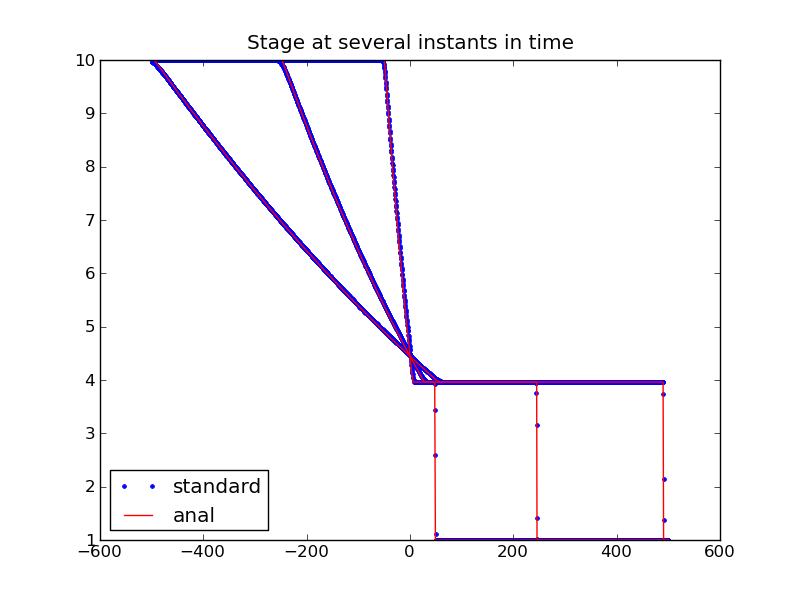
\includegraphics[width=0.9\textwidth]{stage_plot.png}
\end{center}
\caption{Stage results}
\end{figure}


\begin{figure}[h]
\begin{center}
\includegraphics[width=0.9\textwidth]{xmom_plot.png}
\end{center}
\caption{Xmomentum results}
\end{figure}


\begin{figure}[h]
\begin{center}
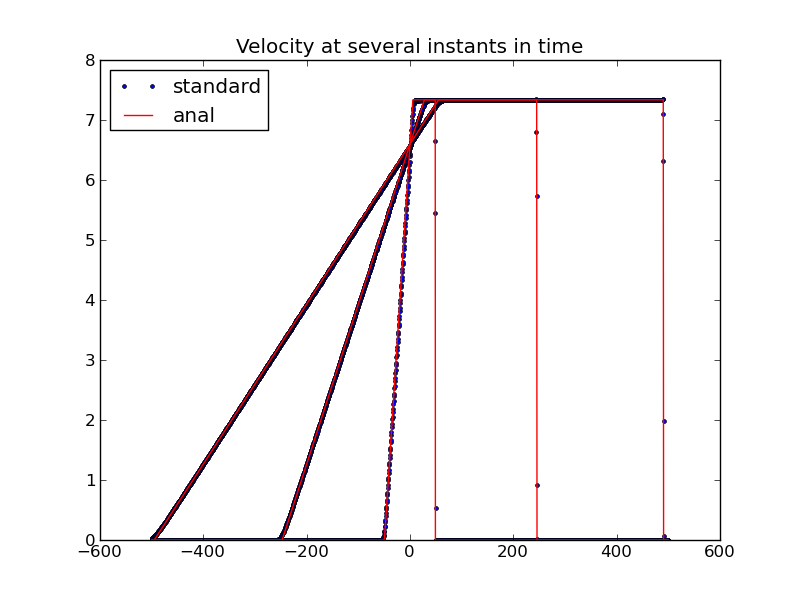
\includegraphics[width=0.9\textwidth]{xvel_plot.png}
\end{center}
\caption{Xvelocity results}
\end{figure}


\endinput
